\label{chap.6}
\section{Why a knowledge graph}
The contingency plans contain exactly the guidance the system must give, but in a form a computer cannot use: tables of free text spread over 30 to 50 pages, with different layouts in different plans. The recommendations also depend on several things at once. The right action for a delayed monsoon depends on the district, the crop, the soil, the season and sometimes the crop stage, and soil types and crops are shared between districts.

A knowledge graph stores such facts as nodes (things) joined by typed edges (relations). It answers multi-hop questions that a flat lookup table cannot, for example "which past seasons in Beed had the same mid-season dry spell, and what soybean yield followed?", and it can keep, on every edge, the plan page the fact came from. The graph needs no data beyond what the preprocessing already produces, and at under a thousand nodes it is small enough to run in memory with NetworkX \cite{hagberg2008exploring} and to export to a graph database such as Neo4j.

\section{Build pipeline}
The graph is built by five scripts, run in order by \texttt{run\_all.py}:

\begin{table}[H]
	\centering
	\caption{Knowledge-graph build steps}
	\label{tab:kgsteps}
	\small
	\begin{tabularx}{\textwidth}{clY}
		\toprule
		\textbf{Step} & \textbf{Script} & \textbf{Output} \\
		\midrule
		1 & \texttt{extract\_pdfs.py} & District profile table; 1,063 condition$\to$action rows; 27 "not applicable" statements \\
		2 & \texttt{label\_seasons.py} & 124 condition labels for past seasons; weather summary for all 260 district-seasons \\
		3 & \texttt{build\_graph.py} & The graph, saved as JSON and GraphML, with summary statistics \\
		4 & \texttt{build\_html\_viewer.py} & An interactive viewer that opens in any browser \\
		5 & \texttt{export\_neo4j.py} & One CSV per node and relation type plus an \texttt{import.cypher} script \\
		\bottomrule
	\end{tabularx}
\end{table}

\section{Extracting the contingency tables}
The extractor uses pdfplumber to read the tables page by page. The plans follow a common ICAR template but are not uniform, so the extractor reads each table's own header instead of assuming fixed columns. The main difficulties and how they were handled:

\begin{itemize}
	\item \textbf{Different column meanings by table type.} Delayed-onset tables have \emph{change in crop / agronomic measures / remarks}; normal-onset and mid-season tables have \emph{crop management / soil nutrient and moisture conservation / remarks}; terminal-drought tables have \emph{crop management / Rabi crop planning / remarks}; and the unusual-rain, flood and extreme-event tables have one column per crop stage (vegetative, flowering, maturity, post-harvest).
	\item \textbf{Wide and two-row headers.} Solapur's tables have 8 to 11 columns with spanned header cells, which are inherited from the left; its \emph{Kharif $|$ Rabi} sub-columns become separate rows, each with its own season. Beed uses two header rows; each column takes its role from whichever row names it.
	\item \textbf{Page breaks.} Text that spills onto the next page is appended to the row it belongs to, and split phrases such as "Delay by 4 weeks" + "2nd week of July" are re-joined.
	\item \textbf{Irrigated situations} (canal, tank, groundwater shortages) are given their own category instead of inheriting the drought heading printed above them.
	\item \textbf{Crop names inside free text,} e.g.\ "Kharif Pearlmillet Preseasonal sugarcane Maize", are found by scanning against the crop vocabulary; a "Rabi" or "Kharif" prefix sets the season.
	\item \textbf{"-do-" and "As above"} cells are resolved from the row above in the same column, and every resolution is recorded. Five dittos have nothing above them and are left flagged.
\end{itemize}

\textbf{Accuracy check.} The first 20 characters of every extracted field were searched for in the cells of the page it came from: of 4,027 fields, 99\% were found verbatim, and the rest are the deliberate joins described above. Beed page 19 and Solapur page 11 were also compared visually with the PDF.

Each recommendation also needs a season. It is taken, in order of preference, from the PDF text itself ("Rabi sorghum", or a Kharif/Rabi sub-column), from the crop calendar for single-season crops (Soybean $\to$ Kharif, Gram $\to$ Rabi), or from the fact that Section~2.1.1 rainfed drought tables concern the Kharif monsoon. Where none applies the season is marked \emph{unspecified}, and such rows are still returned by queries rather than silently dropped.

\section{Season labeller}
\label{sec:labeller}
To connect the plans with real history, every past district-season from 2000 to 2025 is labelled with the conditions it actually experienced, using the plans' own definitions applied to the observed daily rainfall (Table~\ref{tab:labeller}).

\begin{table}[H]
	\centering
	\caption{Rules used by the season labeller}
	\label{tab:labeller}
	\small
	\begin{tabularx}{\textwidth}{p{4.3cm}Y}
		\toprule
		\textbf{Label} & \textbf{Rule} \\
		\midrule
		Onset delayed 2/4/6/8 weeks & Onset = first day from 1 June with a 3-day total $\ge$ 20 mm and no run of $\ge$ 14 rainless days ($<$ 2.5 mm) in the next 30 days. Delay is counted in weeks after 8 June, because the plans equate a 2-week delay with the 4th week of June. \\
		Normal onset, then dry spell & Onset not delayed, and a run of $\ge$ 15 rainless days starting within 30 days of onset. \\
		Mid-season dry spell (vegetative / flowering) & A run of $\ge$ 14 rainless days starting 31--60 / 61--90 days after onset. \\
		Terminal drought & Rainfall from 15 September to 15 October below 50\% of the district's own 2000--2025 mean for that window. \\
		Continuous high rainfall & A 3-day total $\ge$ 150 mm (Kharif), or $\ge$ 64.5 mm in November--February (unseasonal, Rabi). \\
		\bottomrule
	\end{tabularx}
\end{table}

The labeller found 124 condition labels across the 260 district-seasons (Figure~\ref{fig:labels}). The labels agree with known bad years: terminal drought appears in 2014 and 2018, the onset is delayed by about 8 weeks in 2000 and 2015, and Solapur's onset is delayed in 2012. For Beed, for example, 2018 is labelled \emph{normal onset followed by a 25-day dry spell} and \emph{terminal drought} (only 29.7 mm between 15 September and 15 October against a district mean of 141.1 mm), and that season's Kharif rainfall was 37\% below the mean.

\begin{figure}[H]
	\centering
	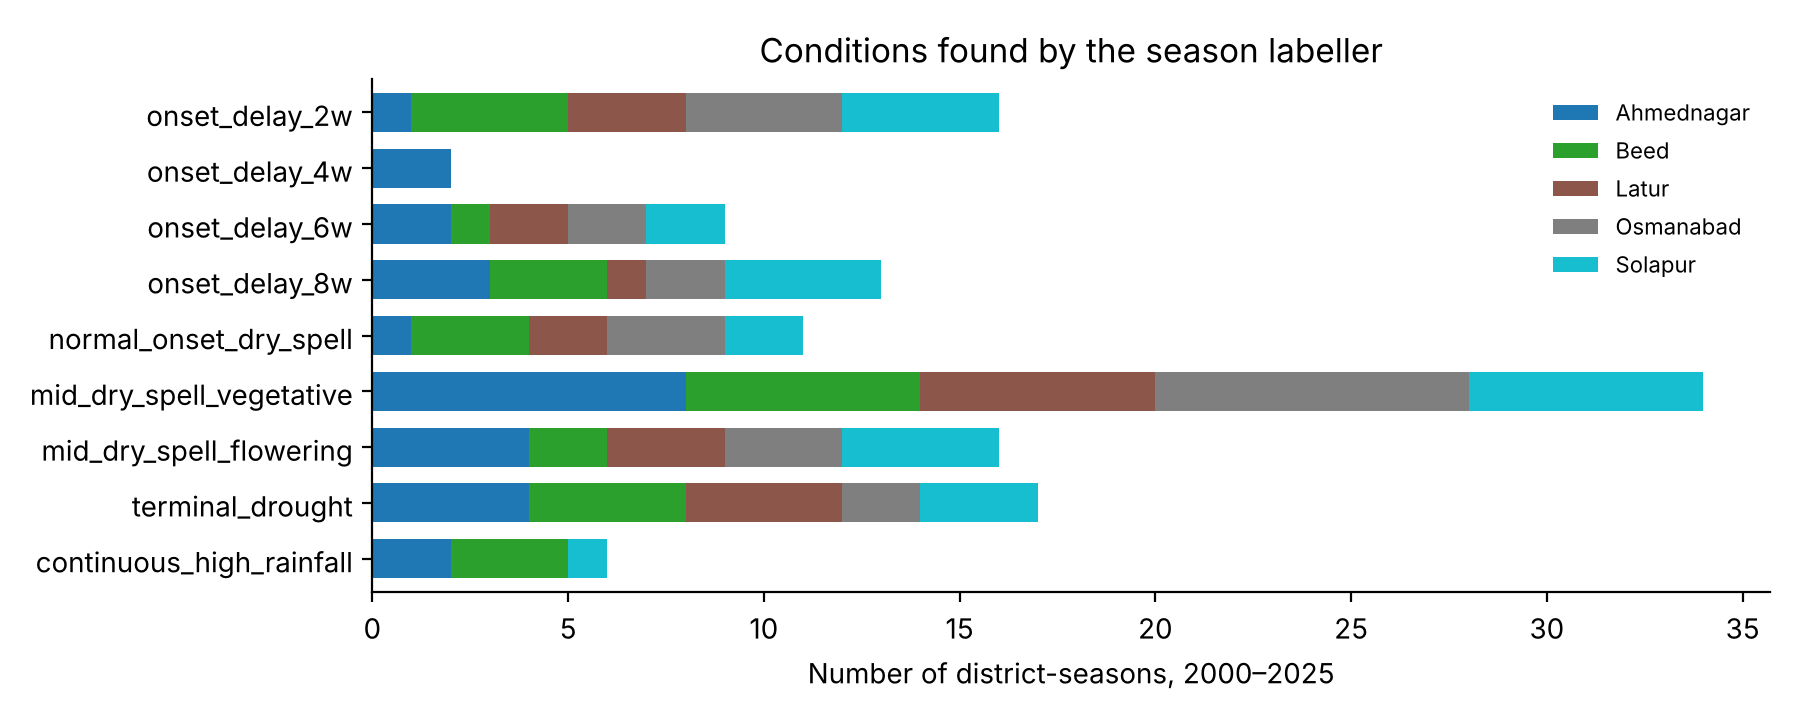
\includegraphics[width=\textwidth]{season_labels.png}
	\caption{Number of district-seasons, 2000--2025, labelled with each condition. Mid-season dry spells during vegetative growth are the most common.}
	\label{fig:labels}
\end{figure}

The labeller is a transparent first version, not a validated drought index, and it also acts as a stand-in for Stage~4: when Stage~4 is built, it will write a file with the same columns and the graph will use it without any change to its schema.

\section{Graph schema}
The finished graph has \textbf{833 nodes} of nine types and \textbf{4,353 edges} of fifteen relation types (Tables~\ref{tab:nodes} and~\ref{tab:edges}).

\begin{table}[H]
	\centering
	\caption{Node types}
	\label{tab:nodes}
	\small
	\begin{tabularx}{\textwidth}{lrY}
		\toprule
		\textbf{Type} & \textbf{Count} & \textbf{What it represents} \\
		\midrule
		District & 5 & The district, with its rainfall normal and irrigated share from the plan \\
		SoilType & 12 & Soil categories from the plans (e.g.\ medium-deep black soil) \\
		Season & 2 & Kharif, Rabi \\
		Crop & 35 & 5 core, 4 extended, 26 fallback/horticulture crops named in the plans \\
		Condition & 7 & Early-season, mid-season and terminal drought; irrigated water shortage; unusual rains; floods; extreme events \\
		ConditionDetail & 24 & Precise sub-types with machine-readable values, e.g.\ onset delayed 4 weeks, 2-week dry spell at flowering, hailstorm \\
		Action & 462 & Unique recommendation texts, split into the plan's own columns \\
		Year & 26 & 2000 to 2025 \\
		SeasonRecord & 260 & One per district, season and year, with that season's weather summary \\
		\bottomrule
	\end{tabularx}
\end{table}

\begin{table}[H]
	\centering
	\caption{Main relation types}
	\label{tab:edges}
	\small
	\begin{tabularx}{\textwidth}{llrY}
		\toprule
		\textbf{Relation} & \textbf{From $\to$ To} & \textbf{Count} & \textbf{Meaning} \\
		\midrule
		RECOMMENDS & ConditionDetail $\to$ Action & 1,063 & One per plan table row; carries district, crop, season, soil, crop stage and \textbf{source page} \\
		APPLIES\_TO\_CROP & Crop $\to$ Action & 702 & The action is for this crop \\
		SOIL\_CONTEXT & SoilType $\to$ Action & 399 & The action is for this soil \\
		SUGGESTS\_CROP & Action $\to$ Crop & 321 & An alternative or Rabi follow-up crop named in the action \\
		HAD\_YIELD & SeasonRecord $\to$ Crop & 788 & The DES area, production and yield that season \\
		EXPERIENCED & SeasonRecord $\to$ ConditionDetail & 124 & The condition the season actually had (from the labeller) \\
		GROWS & District $\to$ Crop & 84 & The district grows this crop \\
		NOT\_APPLICABLE & District $\to$ Condition & 27 & The plan rules this condition out (e.g.\ floods in Beed) \\
		HAS\_SOIL & District $\to$ SoilType & 15 & With area and share \\
		\bottomrule
	\end{tabularx}
	\\[2pt]
	\footnotesize Others: SUBTYPE\_OF (24), IN\_SEASON (20), INCLUDES (6), HAS\_SEASON\_RECORD, IN\_YEAR and OF\_SEASON (260 each).
\end{table}

The core of the graph is the path
\[
\text{Condition} \leftarrow \text{ConditionDetail} \xrightarrow{\text{RECOMMENDS}} \text{Action} \leftarrow \text{Crop},\ \text{SoilType}
\]
filtered by the district and season stored on each RECOMMENDS edge. Around it, the SeasonRecord nodes link the official guidance to 26 years of observed history and yield. Figure~\ref{fig:kgview} shows the interactive viewer.

\begin{figure}[H]
	\centering
	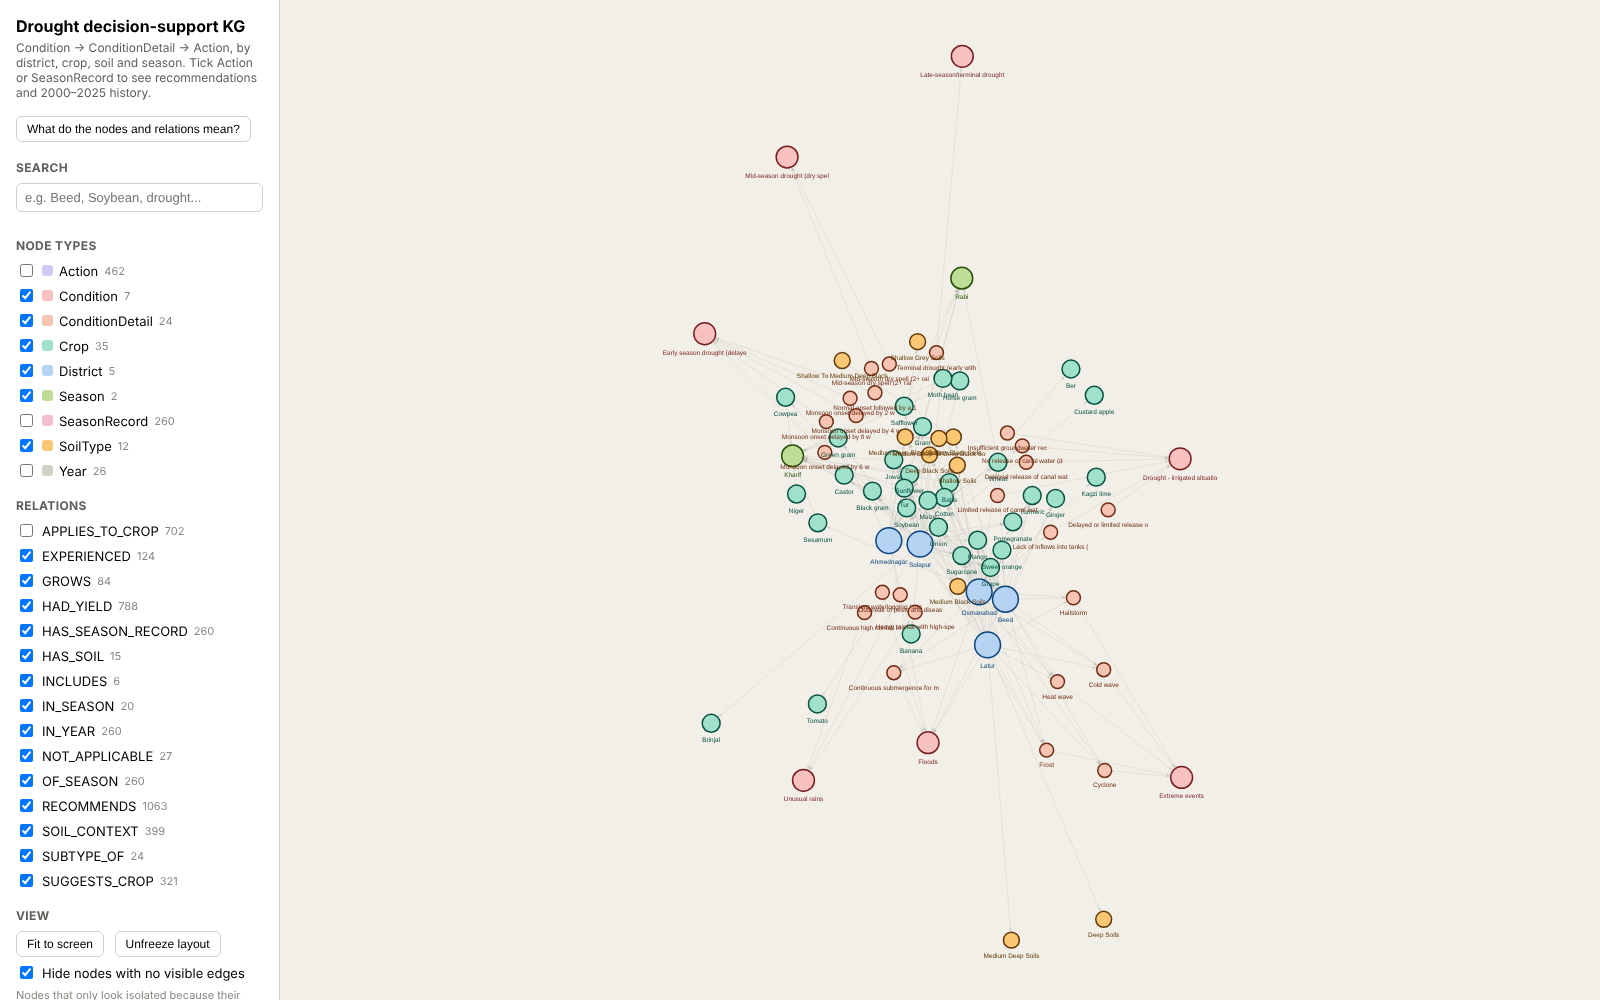
\includegraphics[width=\textwidth]{kg_viewer.png}
	\caption{The interactive knowledge-graph viewer. Node types and relations can be switched on and off in the sidebar; clicking a node or edge shows its details and source. Actions and season records are hidden by default for readability.}
	\label{fig:kgview}
\end{figure}

\section{Querying the graph}
\texttt{kg\_query.py} provides query functions (\texttt{recommend}, \texttt{alternatives}, \texttt{not\_applicable}, \texttt{district\_profile}, \texttt{season\_history}, \texttt{similar\_seasons}, \texttt{yield\_baseline}) and one combined call designed for the LLM layer:

\begin{center}
\texttt{retrieve\_context(G, district, crop, season, condition)}
\end{center}

It returns a single JSON-ready bundle containing the condition's definition, the district profile, the official recommendations with page citations, alternative crops, past seasons with the same condition and the yields that followed, the all-years yield baseline, the plan's "not applicable" statements, and the guardrail text the LLM must obey. The condition can be given as a detail code (\texttt{onset\_delay\_4w}), a category code (\texttt{mid\_season\_drought}) or a category name.

\subsection{Worked example}
For \emph{Beed, Soybean, Kharif}, the graph returns, among others, the following recommendations from the Beed plan:

\begin{table}[H]
	\centering
	\caption{Selected Beed recommendations for soybean returned by the graph}
	\label{tab:example}
	\small
	\begin{tabularx}{\textwidth}{p{4.2cm}Yc}
		\toprule
		\textbf{Condition} & \textbf{Recommended action} & \textbf{Page} \\
		\midrule
		Onset delayed 2 weeks (4th week of June) & No change in cropping & 9 \\
		Onset delayed 4 weeks (2nd week of July) & Soybean (JS-335, MAUS-71) + pigeon pea (BSMR-736, 853, BDN-708, 711) intercrop in 4:2 or 6:3 rows & 10 \\
		Onset delayed 6 weeks (4th week of July) & Shift to pearl millet + pigeon pea in 4:2 or 3:3 rows & 12 \\
		Onset delayed 8 weeks (2nd week of August) & Pearl millet or sunflower (e.g.\ Morden, SS-56, LSH-36) & 13--14 \\
		Normal onset then 15--20 day dry spell & Gap-fill with the same or a short-duration cultivar to keep at least 75\% plant population & 15 \\
		Mid-season dry spell, vegetative & Interculture for weeding and to create a soil mulch; re-sow if plant population is below 50\% & 17--18 \\
		Mid-season dry spell, flowering & Give protective irrigation with sprinkler & 18 \\
		Continuous high rainfall & Drain out excess water; after harvest, shift produce to a safe place and dry it & 24 \\
		\bottomrule
	\end{tabularx}
\end{table}

Alongside these, the graph returns Beed's soil profile (58.9\% shallow black soils, 16\% net irrigated) and the past Kharif seasons labelled with the same condition together with the soybean yield DES recorded for them. This is exactly the material the LLM will be allowed to use.

\section{Neo4j export}
\texttt{export\_neo4j.py} writes one CSV per node and relation type and an \texttt{import.cypher} script that loads them, giving every node a unique key. It can also push the graph directly into a running database. A Cypher query template for the GraphRAG step is included. The export has been generated but not yet loaded into a live Neo4j instance; this is planned together with the GraphRAG layer.

\section{Limitations}
\begin{itemize}
	\item \textbf{The plans date from 2011.} Soil, irrigation and rainfall-normal figures are a single snapshot; Ahmednagar's plan gives no soil percentages and Latur's net irrigated share is not captured.
	\item \textbf{Soil vocabularies differ} between a plan's profile section and its tables, so links between them are made only where names match exactly; several soil groups still need manual checking.
	\item \textbf{Some rows are not captured,} for example rows whose crop cell holds no recognised crop (grasses, tree plantations).
	\item \textbf{Mixed rotation cells} such as "Kharif fallow -- Rabi sorghum / safflower / sunflower" can tag a crop with the wrong season.
	\item \textbf{The labeller uses gridded rainfall,} which smooths extremes, so heavy-rain labels are conservative; it cannot detect pests, hail or canal releases, which therefore come only from the plans.
	\item \textbf{Yield links are missing} for Gram, Wheat, Cotton and Safflower, which are absent from the DES table used.
\end{itemize}

\section{Summary}
The five contingency plans have been converted into a knowledge graph of 833 nodes and 4,353 edges in which every recommendation keeps its source page. A season labeller ties 26 years of observed weather and DES yields to the plans' own condition definitions, and a single query call returns everything the LLM layer will need to give a grounded, cited answer.
